\chapter{基础理论}
\label{chap:theory}

在本文的算法中第一步是通过LTE获取用户的地理位置信息,首先我们会介绍基于LTE标准的设备定位算法,其次参考多篇论文的理论改进LTE定位算法的精度。在LTE定位规范中定义了增强小区ID(英文:Enhanced Cell ID,缩写:E-CellID)\cite{ecellidwiki}和观察到达时差(英文:Observed Time Difference Of Arrival,缩写:OTDOA)\cite{otdoawiki}技术来提高定位的精确度,在标准发布并逐渐实施之后Mebdo等人对LTE定位精度进行了测试,并对提升精度提出了解决方案\cite{medbo2009propagation},在随后的几年中Abeta\cite{abeta2010toward},del Peral-Rosado\cite{del2012achievable}等人也对提升LTE定位精度进行了研究。

在研究人群聚集的突发事件中,我们需要明确人群聚集的规律,于是我们采用了基于社会关系的人群聚集模型,并且对其模型进行深入发掘。早在1995年Helbing等人就提出了针对人群移动的运动模型\cite{helbing1995social}。在此基础之上在2001年Burstedde等人\cite{burstedde2001simulation}提出了二维向量的元胞自动机模型,2002年Kirchner等人\cite{kirchner2002simulation}提出了基于仿生学的元胞自动机模型,二者都对人群聚集模型进行了改进。在2005年Yu等人\cite{yu2005centrifugal}提出了基于离心力的人群移动模型,扩展了研究人群移动模型的思路。

本文提出的算法,在机器学习领域当中是典型的时间序列预测模型,时间序列模型是对历史上的数据进行延展预测,也被称为历史引申预测法。时间序列所反映出来的发展趋势和发展过程,来预测未来可能达到的水平,在本文中我们就是基于收集到的人群移动的数据,来分析在未来时刻是否会发生人群聚集事件,从而提早进行预警并且疏导。

Gradient Boosting Decision Tree(GBDT) \cite{friedman2001greedy}又称为 Multiple Additive Regression Tree(MART)用于计算回归的机器学习算法,GBDT算法是基于决策树模型的机器学习算法,在建模的过程中会尝试使用多棵决策树共同决策,模型当中所有决策树的结论通过数学方法叠加在一起即为最终答案,当把目标函数做变换后,GBDT算法亦可用作解决分类问题或排序问题。

在使用GBDT这种基于监督学习的算法之后,我们尝试使用无监督的自学习算法进行预测,在本文中我们将使用自编码算法(Autoencoder)\cite{bengio2009learning}进行预测。自动编码器是一个人工神经网络用于无监督学习的高效编码\cite{liou2008modeling}\cite{liou2014autoencoder},自动编码器的目的是学习用于一组数据的编码,通常被用于降维。现在自动编码器概念已经越来越广泛地用于学习数据的生成模型\cite{kingma2013auto}。

\section{基于LTE的定位技术}

在3GPP LTE Release 9标准当中,针对设备定位问题定义了如下几种定位方案:
\begin{enumerate}
    \item 基于下行链路的观察到达时间技术(OTDOA)
    \item 增强小区ID技术(E-CellID)
    \item 辅助全球定位系统技术(A-GNSS)
\end{enumerate}

下面我们将分别对比这几种技术的性能,以及各自的特点。

\subsection{OTDOA技术}

OTDOA工作过程如下:移动位置服务中心(英文:Serving Mobile Location Center,缩写:ELMC)通过定位协议层请求OTDOA测量:使用来自用户设备的一组参考信号时间差(英文:Reference Signal Time Difference,缩写:RSTD)测量。与该请求一起,用户设备接收辅助数据。该辅助数据提供小区(enodeB)的列表及其定位参考信号(英文:Positioning Reference Signal,缩写:PRS)参数,包括BW,周期等。

\begin{figure}[!htp]
  \centering
  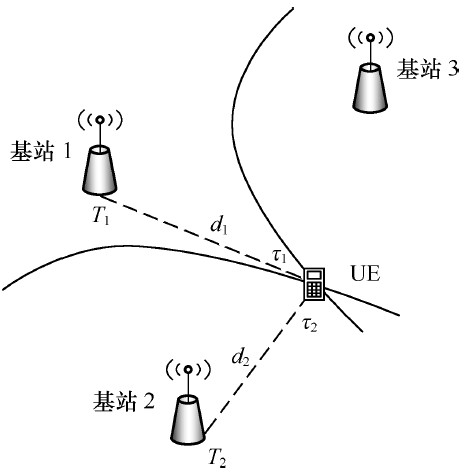
\includegraphics[width=0.6\textwidth]{chap2/otdoa}
  \bicaption[fig:otdoa]{OTDOA技术}{OTDOA技术}{Fig.}{OTDOA}
\end{figure}

然后,用户设备在给定的时间段(通常高达PRS信号的8或16个周期)内继续执行这些测量步骤。这些测量内容包括估计来自每个小区的定位参考信号之间的精确时间偏移,然后,它向移动位置服务中心报告这些估计的时间差以及测量质量。

最后移动位置服务中心通过使用这些时间差以及小区位置和发射时间的偏移量来计算出用户设备的位置。

位置计算基于多边形方法,通过该多边形方法找到双曲线的交点,其中一对单元的双曲线对应于两个具有相同参考信号时间差的一组点。 OTDOA定位方法在图\ref{fig:otdoa2}中示出,其中用户设备正在从eNodeB接收DL信号并且执行RSTD测量$\tau_{1,2}$,$\tau_{1,3}$和$\tau_{2,3}$其形成三个相交的双曲线带,其宽度表示参考信号时间差测量结果的不确定性。参考信号时间差测量的等效距离分别为$d_{1,2}$,$d_{1,3}$和$d_{2,3}$。假设用户设备位于系统中的$(x\qquad y)^T$中,并且eNodeB分别位于$(x_{1}\qquad y_{1})^T$,$(x_{2}\qquad y_{2})^T$和$(x_{3}\qquad y_{3})^T$处,最小二乘法找到二维(2-D)坐标$(x\qquad y)^T$如下。

{\setlength\abovedisplayskip{15pt}
\setlength\belowdisplayskip{15pt}
\begin{eqnarray}
    \label{eq:hyperbolic}
    \sqrt{(x_{1}-x)^2+(y_{1}-y)^2}-\sqrt{(x_{2}-x)^2+(y_{2}-y)^2}=\widehat{d}_{1,2}-\Delta d_{1,2} \nonumber \\
    \sqrt{(x_{2}-x)^2+(y_{2}-y)^2}-\sqrt{(x_{3}-x)^2+(y_{3}-y)^2}=\widehat{d}_{2,3}-\Delta d_{2,3}  \\
    \sqrt{(x_{3}-x)^2+(y_{3}-y)^2}-\sqrt{(x_{1}-x)^2+(y_{1}-y)^2}=\widehat{d}_{1,3}-\Delta d_{1,3} \nonumber
\end{eqnarray}}

其中$\Delta d_{i,j}$是小区$i$和$j$的发射时间差的等效距离(当两个小区完全同步时,即$\Delta d_{i,j} = 0$,对于异步系统则有$\Delta d_{i,j} \ne 0$,例如异步模式的LTE)。满足等式\ref{eq:hyperbolic},需要根据信号源位置和偏移的精确信息来找到用户设备坐标。确定所需的精度是非平凡的。 OTDOA的优点是不需要eNodeB和用户设备之间的同步。

OTDOA定位技术,要求至少要有三个基站才能对用户设备进行定位。

\begin{figure}[!htp]
  \centering
  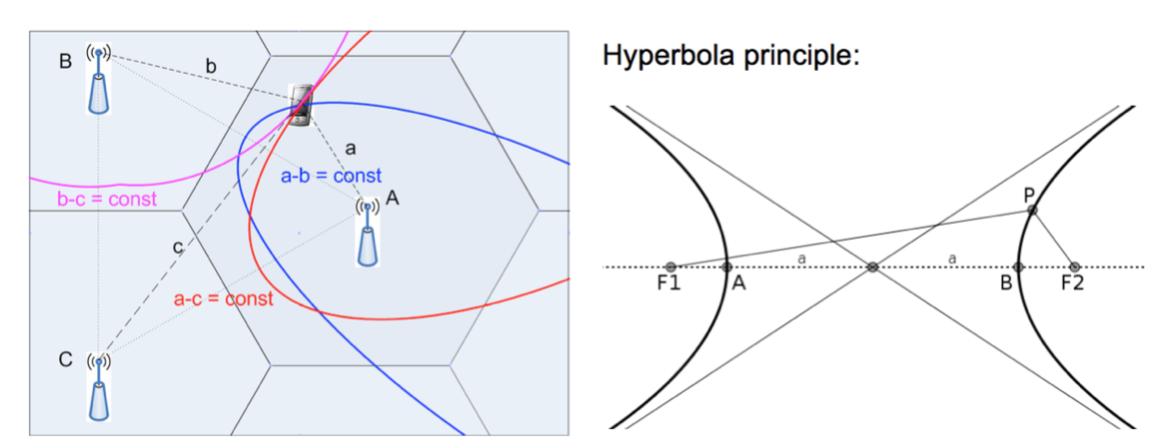
\includegraphics[width=0.8\textwidth]{chap2/otdoa2}
  \bicaption[fig:otdoa2]{OTDOA计算}{OTDO计算}{Fig.}{OTDOA}
\end{figure}

\subsection{E-CellID技术}

在3G时代可以通过设备的小区ID(Cell ID)\cite{trevisani2004cell}给定服小区ID,用户设备位置与小区覆盖区域具有很强的相关性,小区的形状可以通过预先存储的多边形来描述\cite{adams2003location}。 多边形格式是3GPP\cite{3gpp}中的标准定位报告格式之一,其中多边形被定义为3-15个角的列表,每个角由WGS84系统中编码的纬度和经度表示。 单元边界由连接所有角的不相交多边形线段的集合组成。 假定用户设备在具有一定置信度的多边形内,尽管多边形格式本身不包含置信信息,那么我们就可以认为用户设备在这个小区内,因为不需要测量,所以这是最快的定位用户设备的方法。

在新的3GPP Release9标准中,定义了增强小区ID的技术,使得通过小区定位的精度和性能大大提升。

\begin{figure}[!htp]
  \centering
  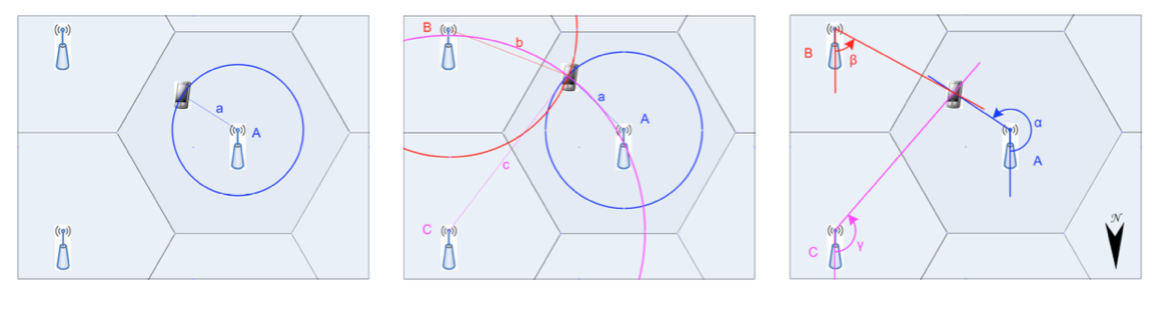
\includegraphics[width=0.8\textwidth]{chap2/ecellid}
  \bicaption[fig:ecellid]{E-CellID技术}{E-CellID技术}{Fig.}{Enhanced Cell ID}
\end{figure}

\begin{figure}[!htp]
  \centering
  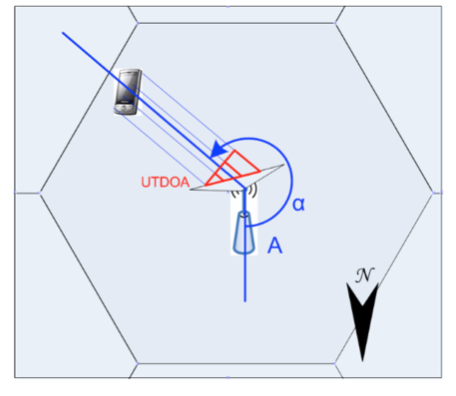
\includegraphics[width=0.4\textwidth]{chap2/ecellid2}
  \bicaption[fig:ecellid2]{E-CellID到达角度}{E-CellID到达角度}{Fig.}{Angle of Arrival}
\end{figure}

E-CID方法利用四个位置信息源:
\begin{enumerate}
    \item 服务小区的CID和相应的地理描述
    \item 服务小区的TA
    \item CID和小区的相应信号强度
    \item 到达角度的大小
\end{enumerate}

接下来,列举一下用于计算E-CellID的三种常见技术。
\begin{enumerate}
    \item \textbf{CID和TA} \\一种常见E-CID方法就是结合地理小区描述,eNodeB位置以及时间计算得到的eNodeB与用户设备之间的距离。TA时间可以通过公式\ref{eq:ta}得到:
    {\setlength\abovedisplayskip{15pt}
    \setlength\belowdisplayskip{15pt}
        \begin{equation}
            \label{eq:ta}
            R_{TA}=\frac{c\cdot TA}{2}
        \end{equation}}
        其中$c$是光速。
    \item \textbf{信号强度} \\ 距离测量还可以从用户设备的信号强度中导出,并且与CID和TA的小区多边形组合。但是当遮蔽效应影响用户手持设备的信号传播时,信号强度变得不准确。这可以通过考虑Okumura-Hata传播模型来解释:
    {\setlength\abovedisplayskip{15pt}
    \setlength\belowdisplayskip{15pt}
        \begin{equation}
            \label{eq:Hata}
            L=L_{0}+10\eta\cdot log_{10}(R)
        \end{equation}}
        其中$L$是以$dB$为单位的路径损耗,$R$是eNodeB与UE之间的距离,$L_{0}$是衰减常数,$\eta$是衰减指数。对公式\ref{eq:Hata}进行微分可得
        {\setlength\abovedisplayskip{15pt}
        \setlength\belowdisplayskip{15pt}
         \begin{equation}
            \label{eq:Hata-diff}
            dL=\frac{10\eta}{ln(10)}\frac{dR}{R} \Leftrightarrow dR=\frac{ln(10)}{10\eta}RdL\approx\frac{ln(10)}{10\eta}R\sigma_{shadow}
        \end{equation}}      
    \item \textbf{到达角度(AOA)} \\ 针对LTE标准中的AOA大小被定义为用户设备相对于参考方向(地理北在顺时针方向上为正)的角度。 与CID和TA方法相比,AOA可以通过减小角度不确定性来提高精度,如图\ref{fig:aoa}所示。 对于给定波束方向$\varphi$和波束宽度$\Phi$,用户设备可能的位置集合是由等式\ref{eq:aoa-eq}给出$(x\qquad y)^T$,其中参数$\gamma$和$\delta$分别在$[0,1]$的范围内变化:
        \begin{figure}[!htp]
            \centering
            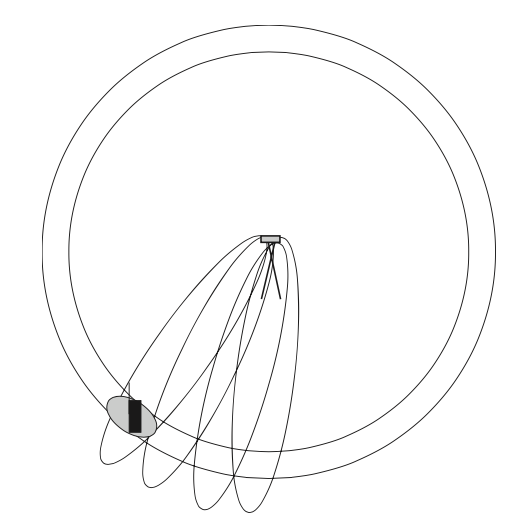
\includegraphics[width=0.8\textwidth]{chap2/aoa}
            \bicaption[fig:aoa]{到达角度示例}{到达角度示例}{Fig.}{Angle of Arrival}
        \end{figure}
        {\setlength\abovedisplayskip{15pt}
        \setlength\belowdisplayskip{15pt}
        \begin{equation}
            \label{eq:aoa-eq}
            \left(\begin{array}{cccc}
                x \\
                y
            \end{array}\right)=(R_{TA}+\Delta R_{TA}(\gamma - \frac{1}{2}))\cdot 
            \left(\begin{array}{cccc}
                sin(\varphi+\Phi(\delta-\frac{1}{2})) \\
                cos(\varphi+\Phi(\delta-\frac{1}{2}))
            \end{array}\right)
        \end{equation}}  
        在LTE标准之前AOA是由具有天线阵列的eNodeB来测量的,但使用LTE标准之后,还可以使用由用户设备上传的预编码器矩阵索引(英文:precoder matrix indices,缩写:PMIs)计算。每个预编码器索引相当于使用“天线波束”。
\end{enumerate}

\subsection{A-GNSS技术}
随着技术的发展人们对移动网络的需求越来越高,促使着定位技术的不断发展,最初的阶段定位技术的需求是可以快速定位,在短时间内响应用户的定位请求,所以提出了基于服务蜂窝小区的定位技术,但是仅仅是基于蜂窝小区的定位技术精度太差,不能满足人们对于精度的需求。于是下一步的发展重点就是提高定位的精确度,在此之后各国大力发展的全球卫星导航系统(英文:Global Navigation Satellite System,缩写:GNSS)定位技术可以精确地定位用户设备,虽然在精度上达到了要求,但是由于需要搜星使初次定位时间(英文:Time To First Fix,缩写:TTFF)过长而显的不那么方便。在全球卫星导航系统当中美国的研究处于领先地位,最早研发并且商用了GPS定位系统,在所有的定位系统单重使用最广为人知并且广泛使用,其他的系统还有欧盟研发的Galileo,俄罗斯研发的Glonass以及我国自主研发的北斗系统。直到LTE标准确定之后辅助GNSS(A-GNSS)技术逐渐被应用起来,辅助GNSS系统是将蜂窝小区定位技术和全球定位系统这两种技术融合产生的,用户的手持设备首先会通过蜂窝小区技术快速的搜索临近的定位卫星,然后使用临近的定位卫星向GNSS系统快速的获得的定位信号并计算出精确地位置,A-GNSS最重要的卖点是可以在保证定位精度的前提之下更快地定位,这是它相对于GNSS系统的最大优势。

\begin{figure}[!htp]
    \centering
    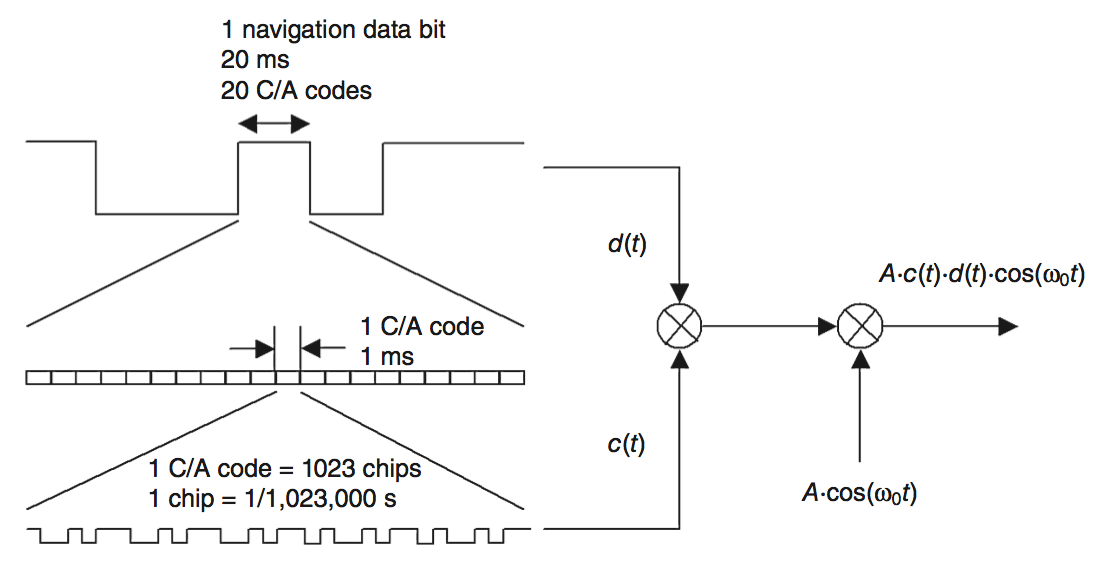
\includegraphics[width=0.8\textwidth]{chap2/gnss-flow}
    \bicaption[fig:gnss-flow]{GPS卫星信号基本特征}{GPS卫星信号基本特征}{Fig.}{The GPS signal structure}
\end{figure}

在这些系统中,只有GPS完全可操作。 来自GPS卫星的发射信号的基本特性如图\ref{fig:gnss-flow}所示。 该信号在L1频率(1175.28MHz)上发射,并且它是码分多址(英文:Code division multiple access,缩写:CDMA)信号,其特征是对于每个卫星唯一的粗伪随机码(英文:coarse acquisition,缩写:C/A)。 关于时间样本$t_{k}$简化模型如公式\ref{eq:tk}所示。

{\setlength\abovedisplayskip{15pt}
\setlength\belowdisplayskip{15pt}
\begin{equation}
    \label{eq:tk}
    y(t_{k})=\sqrt{P}c(t_{k}+\tau_{tr})d(t_{k}+\tau_{tr})e^{j\omega_{tr}t_{k}+\phi}+n(t_{k})
\end{equation}}
其中P是接收的SV信号功率,$c(t)$是卫星的C/A码,以$1/T_{c} = 1.023$MHz的速率切换-1和+1。 C/A码每1ms重复一次。量$\tau_{tr}$是码相位; $d(t)$是-1和+1序列在t时刻的值,以20ms的速率切换; $\omega_{tr}$是未知的多普勒频移;并且$\phi$是未知相位偏移。噪声$n(t)$假定为具有频谱密度$N_{F}k_{B}T_{0}$的白色,其中$N_{F}$是接收机噪声系数,$k_{B} = 1.38\cdot10^{-23} J / K$,$T_{0}$是接收机噪声。其他卫星的干扰在这里没有建模。由于多址干扰对噪声功率增加了0.1dB的能量,所以GPS本质上是噪声限制的CDMA系统。 GPS接收机的任务是找到正确的码相位和多普勒频率,检测数据比特边缘,并执行导航数据解码。当GPS接收机已经获取定时并且解码来自至少四个卫星的导航信号时,它可以确定其位置。 A-GPS接收机试图改善或消除上述一些步骤。为了达到这样的效果,需要从GPS参考接收器的网络收集辅助数据。这些参考接收机位于有利收到信号的位置。接收机连续跟踪可见的SV,解码其消息,并将信息传输到蜂窝网络,以进一步分发到用户设备中的GPS接收机。以这种方式,可以避免解码,并且用户设备中的GPS接收器可以访问完整的导航模型并且校正参数。

A-GPS定位灵敏度和响应时间如表\ref{tab:agps}所示

\begin{table}[!hpb]
    \centering
    \bicaption[tab:agps]{A-GPS对比(假设噪音是5dB)}{A-GPS对比(假设噪音是5dB)}{Table}{A-GPS Comparison}
    \begin{tabular}{@{}cccc@{}} \toprule
        A-GPS类型 & 辅助数据 & 响应时间(s)& 灵敏度(dBm)\\ \midrule
        Stand-alone & FR & 20-40 & -171 \\
        Basic & FR,NM,CT($\approx$2秒) & 8-15 & -178 \\
        Synchronized & FR,NM,AT($\approx$10纳秒) & 1-8 & -185 \\ \bottomrule
    \end{tabular}
\end{table}

\subsection{性能对比}

\textbf{OTDOA}\cite{sun2005signal}定位精度主要取决于RSTD质量和几何形状。实验表明使用10 MHz以及更大的PRS传输带宽的定位效果最佳。在分别将参照物和测量小区噪声设定在-6和-13dB时,达到了标准所需的最小50m测量精度。对于更大范围的实验,RSTD精度约为10m。使用用于同步(1.4MHz)和异步(10MHz)网络的扩展典型城市(ETU)和扩展行人A(EPA)信道模型,来模拟OTDOA测量结果。定位时间分别为1和3个时间单位,并且信号在$N_{prs} = 6$相干累加。在参考文献\cite{medbo2009propagation}中研究了实际测量的传播信道对OTDOA定位的影响,其中高精度和良好校准的信道城市蜂窝LTE场景中的测量数据表明,在规定的时间内,50 \%的测量结果误差在20m左右和95\%的测量误差在63m以内\cite{del2012achievable}。注意,在更困难的无线电环境中,精度可能会进一步降低。

\textbf{E-CellID} 径向精度可以从WCDMA中的RTT定位方法现场试验中得到\cite{wennervirta2010rtt}。 这些结果显示约80m(67\%)和170m(95\%)的径向精度,根据3GPP规范该方法的标称(90\%)测量精度为78m。径向误差的分布如图\ref{fig:ecellid-acc}所示。结果显示传播条件开始主要影响带宽在3.84MHz的WCDMA径向误差。对于LTE,TA的研究结果显示误差在10-40m,这意味着量化误差与用于WCDMA中的RTT定位的量化误差相当。由于LTE系统的带宽通常高于WCDMA的带宽,因此可以得出这样的结论:LTE中的E-CellID略好于WCDMA中的RTT定位精度。

\begin{figure}[!htp]
    \centering
    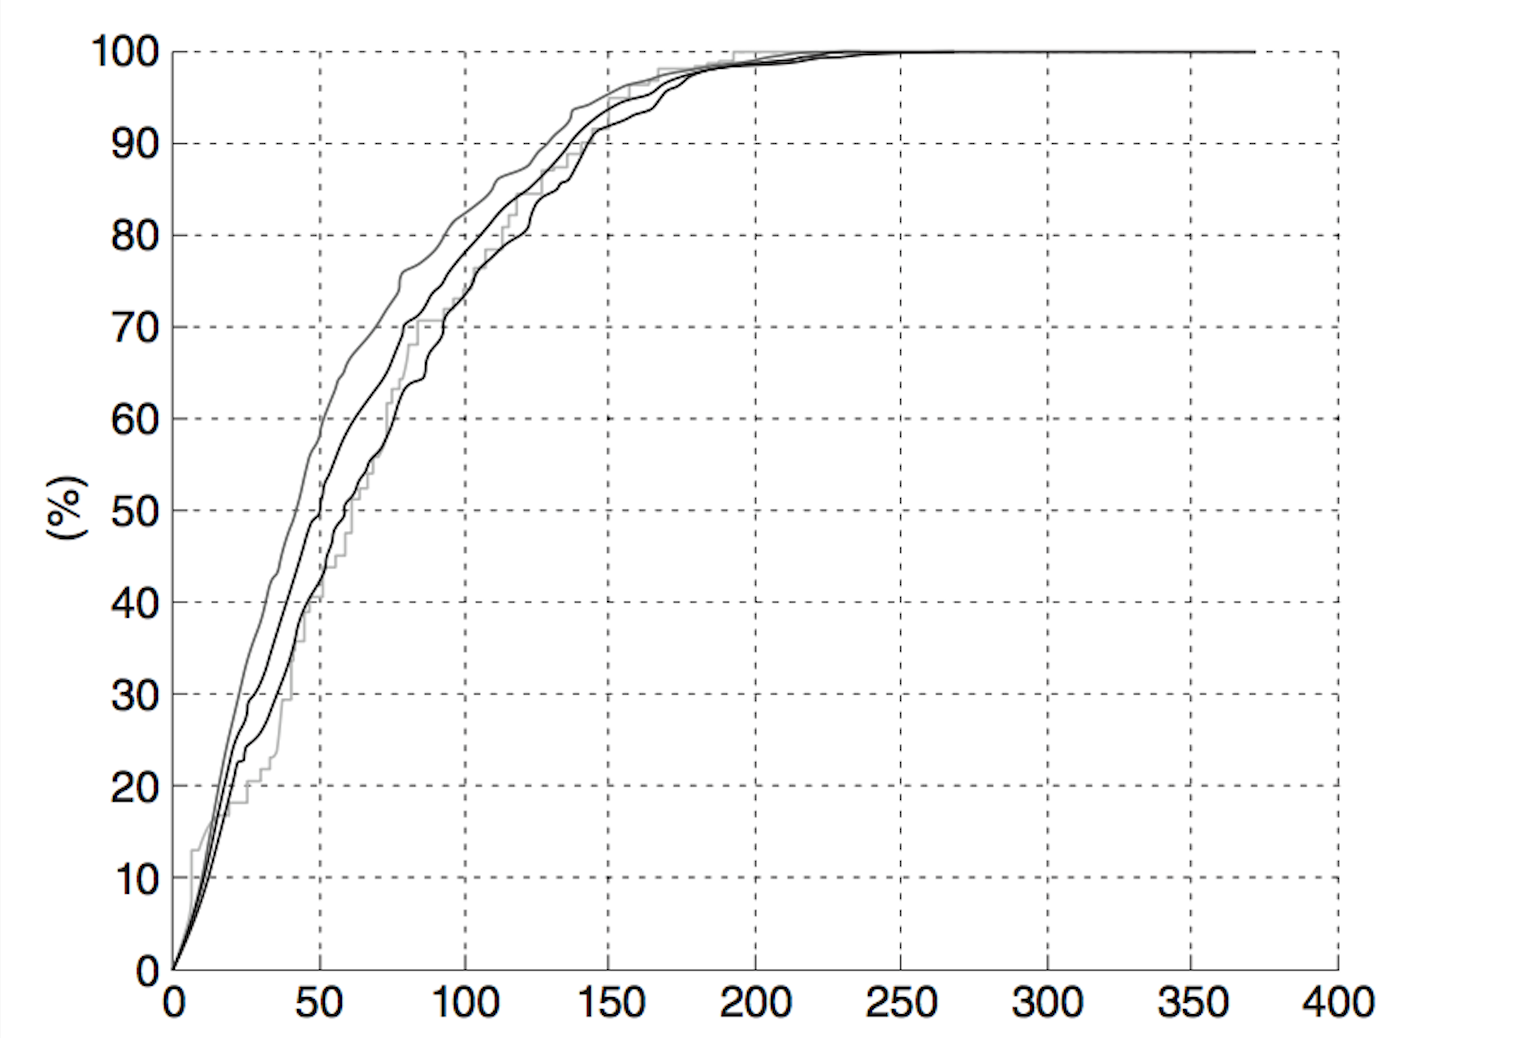
\includegraphics[width=0.8\textwidth]{chap2/ecellid-acc}
    \bicaption[fig:ecellid-acc]{E-CellID绝对误差(米)}{E-CellID绝对误差(米)}{Fig.}{Absolute Radial Error(m)}
\end{figure}

\textbf{A-GNSS} 在许多出版物中已经讨论了A-GPS和A-GNSS的现场性能,并且已知这些方法在空旷野外的条件下非常准确。然而在密集的城市中,由于存在非常高的建筑物导致非直达信号(英文:Non-line-of-sight,缩写:NLOS)传播,使得A-GNSS精度极大的降低,如图\ref{fig:gps-acc}所示。

\begin{figure}[!htp]
  \centering
  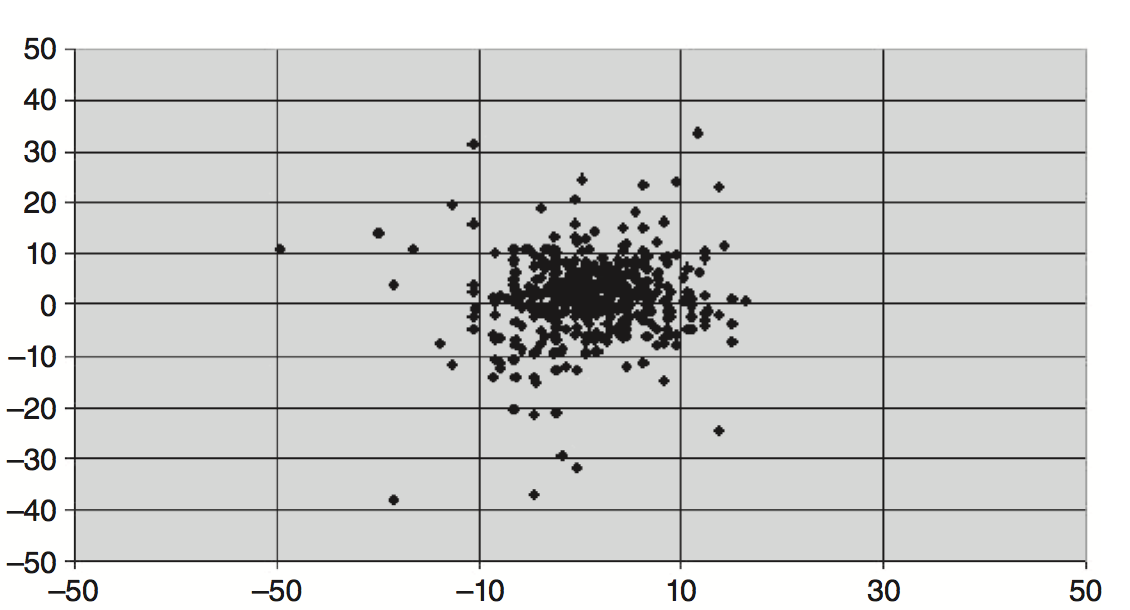
\includegraphics[width=0.3\textwidth]{chap2/gps-nc}
  \hspace{1cm}
  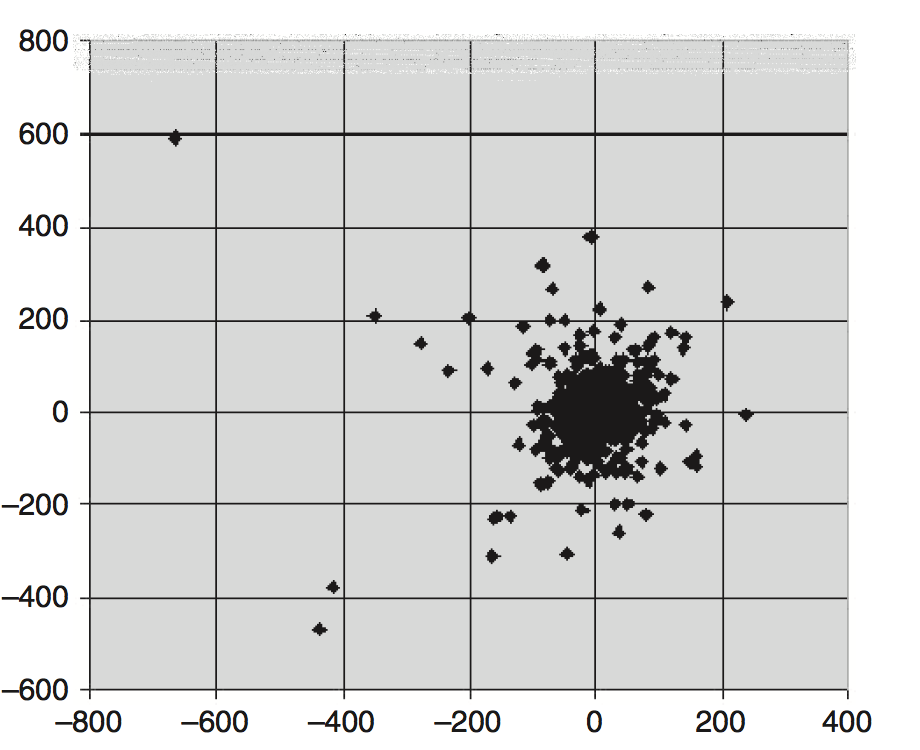
\includegraphics[width=0.3\textwidth]{chap2/gps-cs}
  \bicaption[fig:gps-acc]{A-GNSS乡村和城市环境定位对比}{A-GNSS乡村和城市环境定位对比}{Fig}{A-GNSS accuracy in rural and urban}
\end{figure}

表\ref{tab:lte-comp}中对比了以上几种定位技术的应用场景
\begin{table}[!hpb]
    \centering
    \bicaption[tab:lte-comp]{LTE定位技术应用场景对比}{LTE定位技术应用场景对比}{Table}{Different Positioning Methods in LTE}
    \begin{tabular}{@{}cccccc@{}} \toprule
        定位技术 & 环境限制 & 用户设备影响 & 基站影响 & 系统影响 \\ \midrule
        E-CellID & 无限制 & 小 & 小 & 中 \\
        OTDOA & 仅城市 & 中 & 中 & 中 \\
        A-GNSS & 非室内 & 大 & 小 & 中 \\ \bottomrule
    \end{tabular}
\end{table}

表\ref{tab:lte-comp-acc}中对比了以上几种定位技术的精度
\begin{table}[!hpb]
    \centering
    \bicaption[tab:lte-comp-acc]{LTE定位技术精度对比}{LTE定位技术精度对比}{Table}{Different Positioning Methods Available in LTE}
    \begin{tabular}{@{}cccccc@{}} \toprule
        定位技术 & 可用性 & 响应时间 & 水平方向精度 & 竖直方向精度 \\ \midrule
        E-CellID & 很高 & 低 & 中,$\alpha<1^{\alpha}$ & 无 \\
        OTDOA & 高 & 中 & <100m & 中 \\
        A-GNSS & 高 & 中 & <5m & 中 \\ \bottomrule
    \end{tabular}
\end{table}

\section{人群移动模型}

过去几十年来,人群运动领域越来越受到关注,这是由于以下几个原因:
\begin{enumerate}
    \item 人们的移动性大大增加,即使行走不是最重要的移动形式,但是其他的移动方式都或多或少的与步行有交集(例如,步行到公共汽车,汽车,或到机场终端),此外步行是必要的例如等待和排队,另外步行是最耗时的形式的移动性。模拟行人的意义是可以通过程序辅助建模仿真并减少等待时间。
    \item 大型设施,如主题公园和购物中心,通常由大量人口居住。在密集的人群中,过高的人群密度会容易产生踩踏、交通拥堵和秩序混乱等事故。这需要详细规划“人行道”和人群管理,以避免这种危险的情况。
    \item 例如摇滚音乐会或体育比赛等这种活动常常吸引大量的观众。为了处理这种情况,有必要深入了解人群运动的规律。科学研究是获得这种规律的一个工具,可用于“引导”人群流动,使它们的分布更加均匀,通过引导行人来增加或抑制行人的移动以避免关键区域的峰值流动。
    \item 在紧急情况下,需要建筑物或交通工具中的人员必须尽快的离开事故现场。模拟有助于改善建筑或船只布局并优化疏散效果。
    \item 现代人们不仅仅满足于交通工具的便捷性同时也更改加注重交通工具的安全性。并且交通工具的载重正在逐渐增加,例如飞机(空中客车A380)或船舶(目前计划在船上有超过5000人的大型客船)无论工具数量还是乘客数量都在增加。
    \item 在人群运动中可以观察到许多现象,这些基本原则可以增加对人群动力学的理解。
    \item 最后,群体运动是一个重要议题,它连接到其他几个领域,如社会心理学,交通工程和安全科学。深化这种联系可能得出新的结论超出单一学科的限制。
\end{enumerate}

\begin{figure}[!htp]
    \centering
    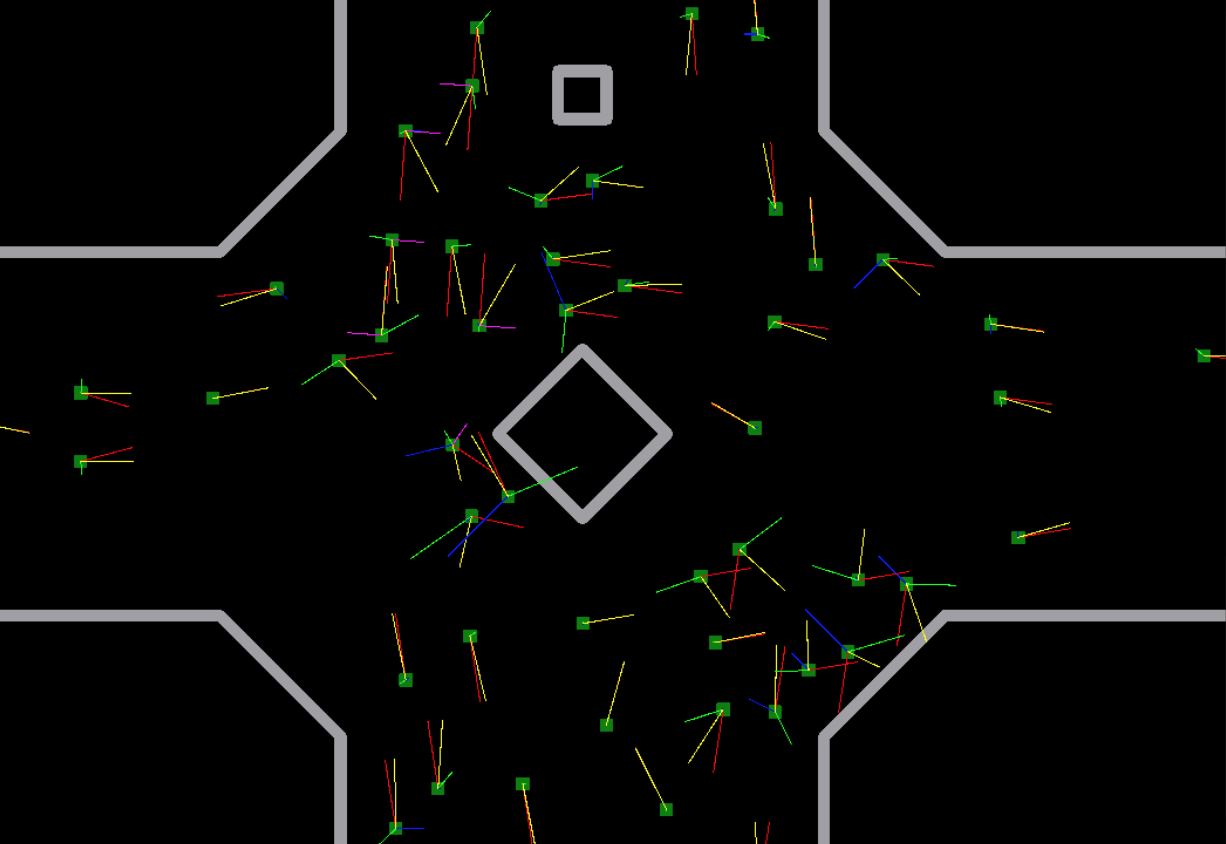
\includegraphics[width=0.8\textwidth]{chap2/pedsim-example}
    \bicaption[fig:pedsim-example]{人群移动模拟软件示例}{人群移动模拟软件示例}{Fig.}{Pedestrian Simulation Example}
\end{figure}

由于所有这些原因,需要彻底调查人群运动的规律及其影响,例如几何布局,环境或程序,特别是在突发紧急事件需要人群撤离的应用场景当中。

行人的运动可以由他们的轨迹表示。假设行人个数为N,如果N个行人的坐标由向量$\overrightarrow{r_{i}}\in ID^{2}$给出,其中$ID = IR$用于空间连续模型,$ID = IN$用于离散模型,新位置$\overrightarrow{r_{i}}'$由$\overrightarrow{r_{i}}+\overrightarrow{v_{i}}$计算出,其中$\overrightarrow{v_{i}}\in ID^{2}$是在$t$时刻的速度,$\Delta t$表示时间步长,于是我们可以在离散模型和连续模型中可以得到公式\ref{eq:move}:

{\setlength\abovedisplayskip{15pt}
\setlength\belowdisplayskip{15pt}
\begin{eqnarray}
    \label{eq:move}
    \overrightarrow{r_{i}}'=\overrightarrow{r_{i}}(t+dt), \qquad \text{在连续模型中} \\
    \overrightarrow{r_{i}}'=\overrightarrow{r_{i}}(t+\Delta t),\qquad \nonumber \text{在离散模型中} 
\end{eqnarray}}

这意味着离散空间可以由二维网格表示,并且网格位点可以由两个坐标表示。确定速度的问题可以细分为三个步骤:路线选择,定向和交互。路线选择需要自主设定战略目标。

在连续模型中,社会关系模型是最早被提出来的,Helbing\cite{helbing2001self}和Hoogendoorn\cite{hoogendoorn2000gas}\cite{hoogendoorn2002microscopic}先后在1995年至2002年几年内对其进行了改进。
该模型可以用公式\ref{eq:social-force}表示:

{\setlength\abovedisplayskip{15pt}
\setlength\belowdisplayskip{15pt}
\begin{equation}
    \label{eq:social-force}
    \frac{d\overrightarrow{x_{i}}(t)}{dt}=\overrightarrow{v_{i}}(t)
\end{equation}}
其中$\overrightarrow{x_{i}}$表示位置,$\overrightarrow{v_{i}}$表示行人$i$的速度。行人$i$受到的力的总和被称为$\overrightarrow{f_{i}}(t)$,$m_{i}$是行人$i$的质量,另外$\overrightarrow{\xi_{i}}$是一些其他的独立变量,最终公式可变形为式\ref{eq:social-force2}

{\setlength\abovedisplayskip{15pt}
\setlength\belowdisplayskip{15pt}
\begin{equation}
    \label{eq:social-force2}
    m_{i}\frac{d\overrightarrow{v_{i}}(t)}{dt}=\overrightarrow{f_{i}}(t)+\overrightarrow{\xi_{i}}(t)
\end{equation}}

用于连续模型过于复杂,所以就相应的产生了离散模型。离散模型能够相对容易的对大型复杂结构进行模拟。离散模型的另一个优势是模拟速度,因为细胞自动机的构造非常适合于高效实施。Nagel-Schreckenberg\cite{nagel1992cellular}模型是模拟道路交通的优秀模型,因此给以给人群运动模型的提供参考。 

\section{决策树模型}

机器学习(英文:Machine Learning)是一门交叉多个领域的科学,机器学习主要涉及到概率论理论、统计学理论、逼近理论、图算法、算法复杂度理论等多门学科,最近二十多年以来计算机的性能逐渐提升,在计算机上存储的数据也越来越多,尤其是近几年随着大数据学科的逐渐发展,机器学习的理论和算法开始逐渐兴起。机器学习算法当中涉及到了众多的统计学知识,众多的机器学习算法都是基于过往的历史资料对未来的趋势进行计算,也有众多算法对现实中的物体进行模糊识别进行分类。通过统计学和概率论当中我们知道很多算法并不能精确地解决现实中的问题,这种情况在机器学习当中尤为明显,在机器学习的数据当中由于存在数量巨大的数据,而这些数据往往很难仅仅通过观察和简单的计算即可发现其中的关联,这样就需要开发出大量的近似算法来解决这种问题。此外机器学习面临的更大的困难是数据处理方面,在传统的计算领域当中数据样本不多,处理起来较为容易而机器学习算法往往需要处理海量的数据这样促进了大数据领域和云计算的发展,所以这些方向也是机器学习领域重要的研究课题。机器学习的应用场景很多,最主要的应用领域还是在数据挖掘当中,这个方向能够提升商品销量为市场提供给更有效地决策,另一个重要领域是计算机视觉,传统的算法很难理解图像中的信息诸如人脸、情绪、运动等信息,而机器学习可以通过处理人工标注的数据,训练出自己可以理解的模型,在这模型之上即可理解这些内容,还有其他重要的研究领域当中可以使用机器学习算法例如生物特征、搜索引擎、语音识别等领域。决策树模型是一种非常重要的机器学习算法。

\begin{figure}[!htp]
    \centering
    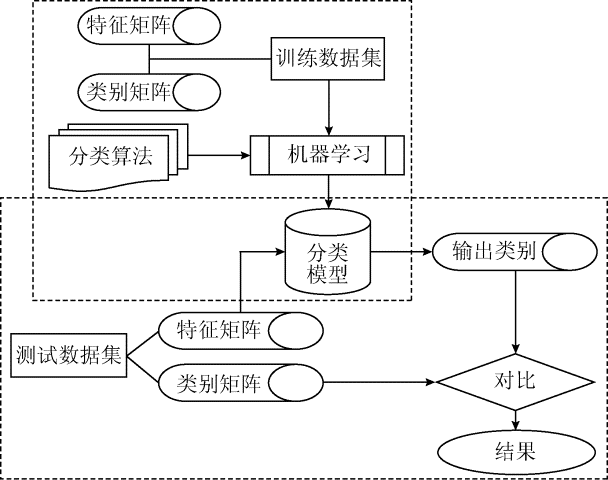
\includegraphics[width=0.8\textwidth]{chap2/ml-example}
    \bicaption[fig:ml-example]{机器学习算法示例}{机器学习算法示例}{Fig.}{Machine Learning Example}
\end{figure}

决策树\cite{quinlan1986induction}通过类似流程图的结构,将其中每个内部节点都视为属性上的测试(例如,抛硬币是正面朝上还是背面朝上),每个分支都被表示为测试的结果,并且每个分支的所有叶节点都被表示为标签。从根节点到叶子节点的路径表示分类规则。在决策模型分析的过程中,决策树以及其密切相关的分布工具被用作可视化和分析决策的工具,用来计算预期值(或预期效用)。

\begin{figure}[!htp]
    \centering
    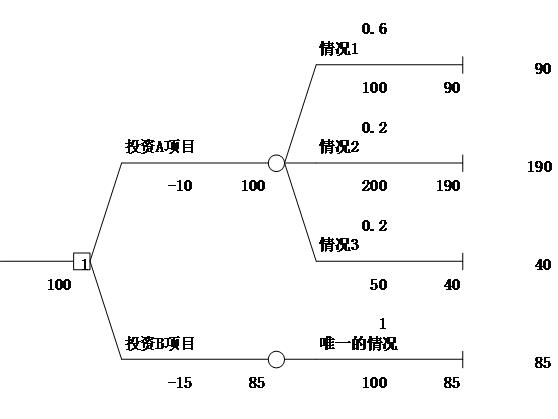
\includegraphics[width=0.8\textwidth]{chap2/decision}
    \bicaption[fig:decision]{决策树模型示例}{决策树模型示例}{Fig.}{Decision Tree Example}
\end{figure}

决策树模型由以下3种类型的节点组成:
\begin{enumerate}
    \item 决策节点 - 通常由正方形表示
    \item 机会节点 - 由圆圈表示
    \item 端节点 - 由三角形表示
\end{enumerate}


决策树通常用于业务研究和业务管理。如果在实践中,必须作出在线在不完全信息情况下决定,不用于重新计算中,决策树应该用于配合概率模型或在线选择算法实现最好的结果。决策树的另一个用途是作为计算条件概率的工具。决策树是一个适合于数字和名义 (离散数据,变量只在有限的一组目标值的结果),能够读取数据的集合,提取的一些数据载于规则。在分类问题中使用决策树模型有很多优点。决策树是不复杂、 简单易用、 高效。决策树可以处理的数据与不相关的特征,并可以方便地构造规则。规则往往容易解释和理解。决策树模型也有一些缺点,比如处理缺失数据、 过度拟合与忽略数据集,如属性间相关性的难度。

决策树学习模型是数据挖掘中常用的方法。在决策树学习模型,每个决策树用来表示树的结构,和其分支机构用于对分类类型的对象特征。每个决策树可以测试原始数据分割。此过程可以递归地修剪树木。递归过程是完整的可能没有进一步分区时或在单个类可以应用到一个分支时。另外,随机森林分类器将许多决策树来提高分类精度结合起来。


决策树通常用于操作研究和操作管理当中,如果在实践中决策必须在不完整的信息情况下在线进行决策而不是用来进行召回计算,则决策树应当与概率模型或者在线选择算法一起使用才能发挥最好的效果。决策树的另一种用途是作为用于计算条件概率的工具。决策树适用于数值型和标称型(离散型数据,变量的结果只在有限目标集中取值),能够读取数据集合,提取一些列数据中蕴含的规则。在分类问题中使用决策树模型有很多的优点,决策树计算复杂度不高、便于使用、而且高效,决策树可处理具有不相关特征的数据、可很容易地构造出易于理解的规则,而规则通常易于解释和理解。决策树模型也有一些缺点,比如处理缺失数据时的困难、过度拟合以及忽略数据集中属性之间的相关性等。

决策树学习模型是数据挖掘中一个常用的方法。在决策树学习模型中每个决策树都用来表征一种树型结构,用它的分支来对该类型的对象特征进行分类。每个决策树可以通过对原始数据的分割进行数据测试。这个过程可以递归的对树进行修剪。当不能再进行分割或一个单独的类可以被应用于某一分支时,递归过程就完成了。此外,随机森林分类器将许多决策树结合起来以提升分类的正确率。

一般情况下生成决策树的需要经历特征选择、生成算法和剪枝算法三个步骤:
\begin{enumerate}
    \item 特征选择:特征选择是指从训练数据中众多的特征中选择一个特征作为当前节点的分裂标准,如何选择特征有着很多不同量化评估标准标准,从而衍生出不同的决策树算法。
    \item 决策树生成: 根据选择的特征评估标准,从上至下递归地生成子节点,直到数据集不可分则停止决策树停止生长。 树结构来说,递归结构是最容易理解的方式。
    \item 剪枝:决策树容易过拟合,一般来需要剪枝,缩小树结构规模、缓解过拟合。剪枝技术有预剪枝和后剪枝两种。
\end{enumerate}

影响决策树分类效果的最重要的部分就是特征选择这一步骤,而且特征选择是之后生成算法和剪枝算法的基础,在决策树算法当中一个恰当的特征被选择作为判断节点之后可以直接影响到决策树递归的深度,相应的如果选择不当的特征会导致决策树深度增加相应的计算量会显著提升严重影响算法的时间复杂度。决策树模型的最理想的状况是通过分类将不同类别的数据集合分配道不同的组当中,在选择特征时最重要的衡量指标就是数据集的纯度,纯度越高说明数据分类是错分的也就越少,所以我们下面将针对几种常见的纯度函数一一介绍。

\begin{enumerate}
    \item \textbf{信息增益} \\ 
    在信息理论和机器学习中,信息增益是Kullback-Leibler发散的同义词,然而在决策树的上下文中,信息增益有时与互信息同时使用,互信息是一个变量的单变量概率分布的Kullback-Leibler发散的期望值与给定另一个变量的该变量的条件分布的期望值,在构建决策树是我们根据给定的样本数据集选择某个特征值作为树的节点。下面我们从数学的角度来分析信息增益的计算过程,不妨设我们有$c$种数据不规则的分布在数据集$D$中。在数据集$D$可以通过公式\ref{eq:entropy1}计算出该数据中的信息熵:
    {\setlength\abovedisplayskip{15pt}
    \setlength\belowdisplayskip{15pt}
    \begin{equation}
        \label{eq:entropy1}
        Info(D)=-\sum_{i=1}^{c}p_{i}log_{2}(p_{i})
    \end{equation}}
    其中$D$表示训练数据集,$c$表示数据类别数量,$p_{i}$表示类别$i$样本占总样本的数量。
    对应数据集$D$,选择特征$A$作为决策树判断节点时,在特征$A$作用后的信息熵的为$Info(D)$,计算如公式\ref{eq:entropy2}所示:
    {\setlength\abovedisplayskip{15pt}
    \setlength\belowdisplayskip{15pt}
    \begin{equation}
        \label{eq:entropy2}
        Info_{A}(D)=-\sum_{i=1}^{k}\frac{|D_{i}|}{|D|}\times Info(D)
    \end{equation}}  
    其中$k$表示样本$D$被分为$k$个部分。
    信息增益表示数据集$D$在特征$A$的作用之后,其信息熵的减少值。公式如\ref{eq:entropy3}所示:
    
    {\setlength\abovedisplayskip{15pt}
    \setlength\belowdisplayskip{15pt}
    \begin{equation}
        \label{eq:entropy3}
        Gain(D)=Info(D)-Info_{A}(D)
    \end{equation}}

    \item \textbf{基尼指数}\\ 
    基尼指数是另一种数据的不纯度的度量方法,其公式为\ref{eq:gini1}:
    
    {\setlength\abovedisplayskip{15pt}
    \setlength\belowdisplayskip{15pt}
    \begin{equation}
        \label{eq:gini1}
        Gini(D)=1-\sum_{i=1}^{c}p_{i}^2
    \end{equation}}

    在极端情况也数据集$D$包含一种类型的数据,那么此时基尼系数达到最小值0,这是我们加入选取属性这一变量,不妨设为$A$,进一步推导数据集$D$的基尼指数为\ref{eq:gini2}:
    
    {\setlength\abovedisplayskip{15pt}
    \setlength\belowdisplayskip{15pt}
    \begin{equation}
        \label{eq:gini2}
        Gini_{A}(D)=\sum_{i=1}^{k}\frac{|D_{i}|}{|D|}Gini(D_{i})
    \end{equation}}
    其中$k$表示样本$D$被分为$k$个部分,数据集$D$分裂为$k$个$D_{i}$数据集。对于特征选取,需要选择最小的分裂后的基尼指数。也可以用基尼指数增益值作为决策树选择特征的依据。公式如\ref{eq:gini3}所示:
    
    {\setlength\abovedisplayskip{15pt}
    \setlength\belowdisplayskip{15pt}
    \begin{equation}
        \label{eq:gini3}
        \Delta Gini(A)=Gini(D)-Gini_{A}(D)
    \end{equation}}
    \item \textbf{方差减少} \\
     在目标变量是连续的的情况下经常采用方差降低算法,在在应用之前许多其他参数进行离散化。节点$N$的方差减少被定义为用于在该节点处的划分而导致的目标变量$x$的总方差减少:
    
    {\setlength\abovedisplayskip{15pt}
    \setlength\belowdisplayskip{15pt}
    \begin{equation}
        \label{eq:vr}
        I_{V}(N)={\frac {1}{|S|^{2}}}\sum _{i\in S}\sum _{j\in S}{\frac {1}{2}}(x_{i}-x_{j})^{2}-\left({\frac {1}{|S_{t}|^{2}}}\sum _{i\in S_{t}}\sum _{j\in S_{t}}{\frac {1}{2}}(x_{i}-x_{j})^{2}+{\frac {1}{|S_{f}|^{2}}}\sum _{i\in S_{f}}\sum _{j\in S_{f}}{\frac {1}{2}}(x_{i}-x_{j})^{2}\right)
    \end{equation}}
    其中$S$,$S_{t}$和$S_{f}$分别是样本的集合,为真的样本索引集合,为假的样本索引集合。 式\ref{eq:vr}中的每一个总和是方差估计,但是以不直接引用均值的形式写出。  
\end{enumerate}

接下来介绍剪枝。在分类模型建立的过程中,很容易出现过拟合现象,如图\ref{fig:overfit}所示。过拟合现象是指在模型学习训练当中,训练样本达到了一个非常高的逼近精度,但对检验样本的逼近误差随着训练次数而呈现出先下降后上升的现象。过拟合表现出来的现象就是时训练误差很小,但是检验误差很大,无法用于真实的应用场景。决策树的过拟合现象可以通过剪枝进行一定的修复。剪枝分为预先剪枝和后剪枝两种模式,如图\ref{fig:jianzhi}所示。

\begin{figure}[!htp]
    \centering
    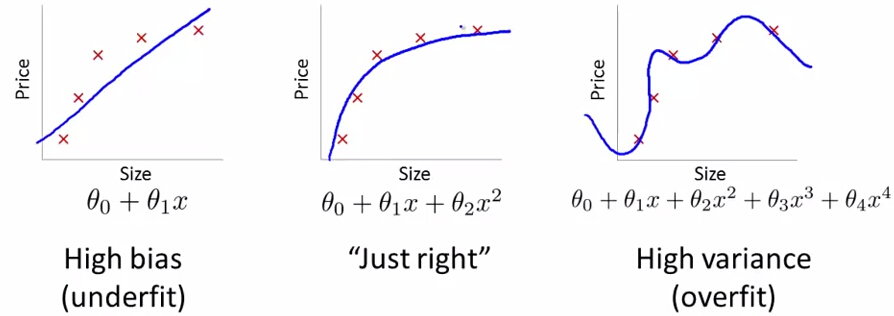
\includegraphics[width=0.8\textwidth]{chap2/overfit}
    \bicaption[fig:overfit]{过拟合示例}{过拟合示例}{Fig.}{Overfit}
\end{figure}

\begin{figure}[!htp]
    \centering
    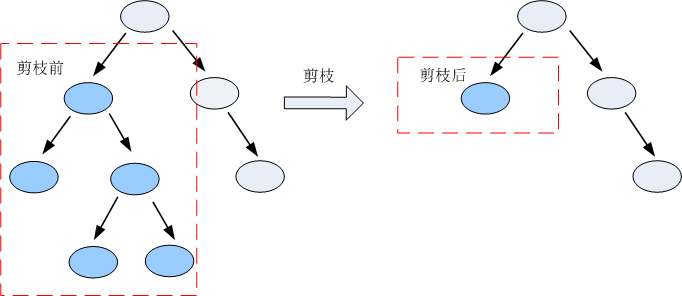
\includegraphics[width=0.8\textwidth]{chap2/jianzhi}
    \bicaption[fig:jianzhi]{决策树剪枝示例}{决策树剪枝示例}{Fig.}{Pruning}
\end{figure}

\begin{enumerate}
    \item 预先剪枝在局册数完全分类训练集之前停止生长树。
    \item 后剪枝允许树完全分类训练集,然后修剪树。
\end{enumerate}

实际上,后剪枝技术应用的更加广泛,因为在真实的环境当中不容易精确地估计何时停止生长树。树修剪的重要步骤是定义用于使用以下方法之一来确定正确的最终树大小的准则:

\begin{enumerate}
    \item 使用来自训练集(称为验证集)的不同数据集,以评估来自树的后修剪节点的效果。
    \item 通过使用训练集来构建树,然后应用统计测试来估计修剪或扩展特定节点是否可能产生超出训练集的改进。
    \begin{enumerate}
        \item 错误估计
        \item 显着性检验(例如卡方检验)
    \end{enumerate}
    \item 最小描述长度原则:使用编码训练集和决策树的复杂度的显式度量,当此编码大小$(size(tree)+ size(misclassifications(tree))$最小化时停止树的增长。
\end{enumerate}
第一种方法是最常用的方法,在这种方法中,可用数据被分成两组示例:用于构建决策树的训练集和用于评估修剪树的影响的验证集,第二种方法也是一种常用的方法。

决策树模型有以下六个方面的优势:

\begin{enumerate}
    \item 决策树易于理解和实现;
    \item 易于通过静态测试来对模型进行评测;
    \item 数据无需预处理过程;
    \item 对于数据的属性没有明确要求;
    \item 逻辑表达式更加直观易于推到;
    \item 相对短的时间内能够对大型数据源做出效果良好的结果;
\end{enumerate}

但是相应的决策树模型有以下方面的劣势:

\begin{enumerate}
    \item 对于各类别样本数量不一致的数据,在决策树当中信息增益的结果往往偏向于那些具有更多数值的特征。
\end{enumerate}

学习最优决策树的问题被认为是在最优性的NP完全问题,甚至是简单的概念。因此实际的决策树学习算法往往基于启发法,例如贪心算法等,其中在每个节点处取局部最优结果,但是不能保证返回全局最优决策树。为了减少局部最优性的贪心效应,需要提出一些更优化的方法,例如双信息距离树(英文:Dual Information Distance,缩写:DID)\cite{ben2014efficient}。决策树学习模型可以创建不能从训练数据推广的过度复杂树,这就是所谓的过拟合,要避免这个问题剪枝机制是必要的。例如XOR,奇偶校验或多路复用器问题。在这种情况下生成的决策树将变得非常大。解决问题的方法包括改变问题域的表达方式或使用更具表现力的模型(如统计关系学习或归纳逻辑编程)的学习算法。对于包括具有不同级数的分类变量的数据,决策树中的信息增益偏向于具有更多级别的那些属性。然而有条件的推理方法避免了有偏见的预测器选择的情况。

\section{GBDT预测算法}

Gradient Boosting Decistion Tree(GBDT)主要由三个概念组成:

\begin{enumerate}
    \item 决策树算法 Regression Decistion Tree
    \item 梯度迭代 Gradient Boosting
    \item 迭代收缩 Boosting Shrinkage
\end{enumerate}
它在被提出之初就和支持向量机(英文:Support Vector Machine, 缩写:SVM)一起被认为是泛化能力较强的算法。决策树在上一节中已经充分介绍过了,下面我们将详细的介绍梯度迭代算法和迭代收缩过程。

梯度迭代(英文:Gradient Boosting)\cite{friedman2002stochastic}是用于回归和分类问题的机器学习算法,其以弱预测模型(通常是决策树)的集合的形式产生预测模型。它与其他迭代方法一样采用阶段式的方式构建模型,并且允许任意可微分损失函数的优化来概括它们。梯度迭代的想法源于Leo Breiman\cite{breiman1997arcing}在1997年发表的文章,文章中提到增强可以被视为开销稳定的函数的优化算法。回归梯度提升算法随后由Jerome H. Friedman\cite{friedman2001greedy}\cite{friedman2002stochastic}最先提出,Llew Mason\cite{mason1999boosting}Jonathan Baxter,Peter Bartlett和Marcus Frean等人提出了更通用梯度迭代算法,通过迭代地选择指向负梯度方向的函数(弱假设)来优化函数空间上的成本函数。这种迭代功能梯度算法促进了在机器学习和统计等领域中在回归和分类的基础之上迭代算法的发展。

\begin{figure}[!htp]
    \centering
    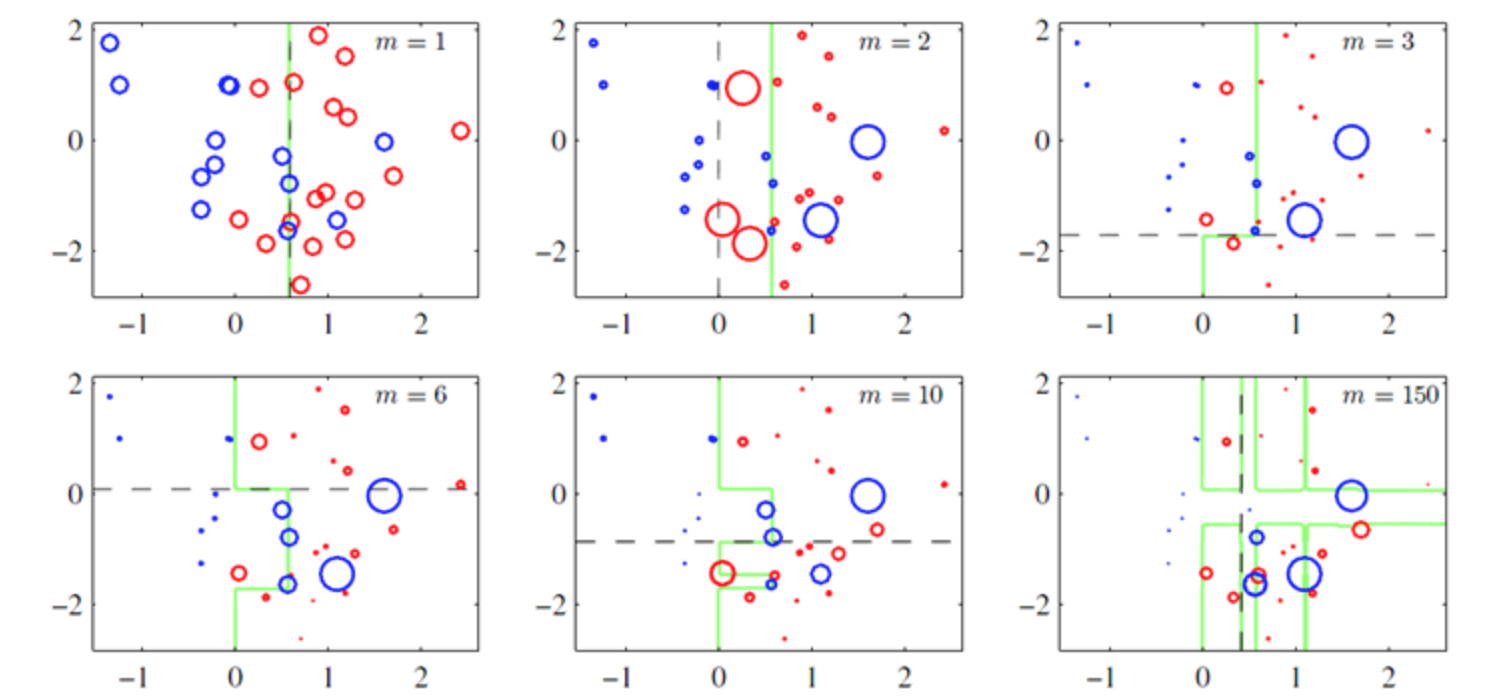
\includegraphics[width=0.8\textwidth]{chap2/boosting-example}
    \bicaption[fig:boosting-example]{Boosting 算法示例}{Boosting 算法示例}{Fig.}{Boosting Example}
\end{figure}

迭代可以用公式\ref{eq:boosting}表示,如图\ref{fig:boosting}:

{\setlength\abovedisplayskip{15pt}
\setlength\belowdisplayskip{15pt}
\begin{equation}
    \label{eq:boosting}
    Y_{M}(x)=sign(\sum_{m}^M\alpha_{m}y_{m}(x))
\end{equation}}

\begin{figure}[!htp]
    \centering
    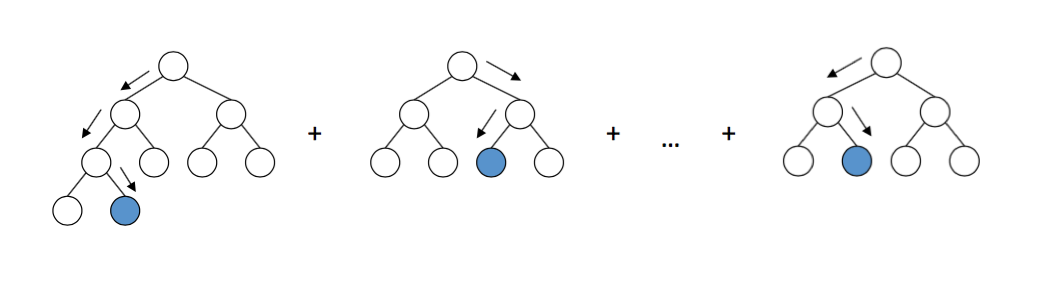
\includegraphics[width=0.8\textwidth]{chap2/boosting}
    \bicaption[fig:boosting]{Boosting计算过程}{Boosting计算过程}{Fig.}{Boosting}
\end{figure}Marcus

\subsection{梯度迭代}

梯度增强涉及三个要素,分别是:要优化的损失函数、一个弱学习者做出预测以及增加弱学习者加性模型的最小化损失函数。对于损失函数来说,使用的损耗函数取决于要解决的问题的类型,它必须是可区分的,但是支持许多标准丢失函数,例如回归可以使用平方误差,并且分类可以使用对数损失。梯度提升框架的益处在于不必为可能想要使用的每个损失函数导出新的提升算法,相反其是可以使用任何可微分损失函数的通用足够的框架。决策树用作梯度提升中的弱学习者,特别地,使用输出分割的实际值并且其输出可以被加在一起的回归树,允许添加随后的模型输出并且在预测中“校正”残差,树以贪婪的方式构建,基于诸如吉尼等纯度分数选择最佳分割点,或者使损失最小化,通常以特定方式约束弱学习者,这是为了确保学习者保持弱势,但仍然可以贪婪的方式建造。最后是添加模型,每次添加一个树,并且模型中的现有树不会更改,梯度下降过程用于最小化添加树时的损失,传统上,梯度下降用于最小化一组参数,在计算误差或损失之后,更新权重以最小化该误差。除了参数我们有弱学习器子模型或更具体地决策树。在计算损失之后,为了执行梯度下降过程,我们必须向模型添加一个树以减少损失。我们这样做通过参数化树,然后修改树的参数,并向右移动。

通常这种方法称为函数梯度下降。像其他迭代方法一样,梯度迭代将弱学习者以迭代方式组合成单个强大的学习者。用最小二乘回归最容易解释,其中学习模型$F$预测出结果$\hat{y} = F(x)$,其中使得均方根$(\hat{y} - y)^2$最小的$y$即为预测结果。

在每个$1 \le m \le M$阶段,梯度升压的每一阶段,可以假定存在一些不完美的模型$F_m$(在开始时,使用弱模型训练出的模型预测出结果$y$)。梯度升高算法不以任何方式改变$F_m$,而是通过构造添加估计函数$h$以提供更好的模型$F_{m + 1}(x)= F_m(x)+ h(x)$的新模型来对其进行改进。在这里需要解决的就是如何找到估计函数$h$。可以用式\ref{eq:fh}表示:

{\setlength\abovedisplayskip{15pt}
\setlength\belowdisplayskip{15pt}
\begin{eqnarray}
    \label{eq:fh}
    F_{m+1}(x)=F_{m}(x)+h(x)=y \nonumber \\
    h(x) = y - F_m(x)
\end{eqnarray}}

\subsection{算法描述}
下面的内容就是用数学的方式来描述Gradient Boosting。
假设我们的模型能够用式\ref{eq:gb1}来表示,$P$由多个参数组成$P = {p_{0},p_{1},p_{2}….}$,$F(x;P)$表示以$P$为参数的关于$x$的函数,这就是我们的预测函数。我们的模型是由多个模型叠加构成,$\beta$表示每个模型的权重,$\alpha$表示模型里面的参数。为了优化$F$,我们就可以优化${\beta,\alpha}$。

{\setlength\abovedisplayskip{15pt}
\setlength\belowdisplayskip{15pt}
\begin{equation}
    \label{eq:gb1}
    F(x;P)=F(x;\{\beta_{m},\alpha_{m}\}_{1}^{M})=\sum_{m=1}^{M}\beta_{m}h{x;\alpha_{m}}
\end{equation}}

我们还是用$P$来表示模型的参数,可以得到$\Phi(P)$表示$P$似然函数,也就是模型$F(x;P)$的损失函数。

{\setlength\abovedisplayskip{15pt}
\setlength\belowdisplayskip{15pt}
\begin{eqnarray}
    \label{eq:gb2}
    P^{*}=argmin(\Phi(P)) \\
    \Phi(P)=E_{y,x}L(y,F(x;P)) \nonumber
\end{eqnarray}}

既然模型$F(x;P)$是可以叠加的,对于参数$P$,我们也可以得到下面的式\ref{eq:gb3}:

{\setlength\abovedisplayskip{15pt}
\setlength\belowdisplayskip{15pt}
\begin{equation}
    \label{eq:gb3}
    P^{*}=\sum_{m=0}^M p_{m}
\end{equation}}

假设当前已经得到了$m-1$个模型,在我们想要得到第$m$个模型的时候,我们首求前$m-1$个模型的梯度。得到最快下降的方向,就是$g_{m}$最快的下降方向。

{\setlength\abovedisplayskip{15pt}
\setlength\belowdisplayskip{15pt}
\begin{equation}
    \label{eq:gb4}
    g_{m}=\{g_{jm}\}=\{[\frac{\partial\Phi(P)}{\partial p_{j}}]_{p=p_{m-1}}\}
\end{equation}}

我们不妨假设前$m-1$个模型是不可变的,我们的关注点是以后模型的建立过程。

{\setlength\abovedisplayskip{15pt}
\setlength\belowdisplayskip{15pt}
\begin{equation}
    \label{eq:gb5}
    P_{m-1}=\sum_{i=0}^{M-1} p_{i}
\end{equation}}

通过不断地迭代我们得到的新的模型,它就在$P$的似然函数的梯度方向。其中$\rho$是在梯度方向上下降的距离:
{\setlength\abovedisplayskip{15pt}
\setlength\belowdisplayskip{15pt}
\begin{equation}
    \label{eq:gb6}
    p_{m}=-\rho_{m}g_{m}
\end{equation}}

最终我们可以通过优化的式\ref{eq:gb7}来得到最优的$\rho$:

{\setlength\abovedisplayskip{15pt}
\setlength\belowdisplayskip{15pt}
\begin{equation}
    \label{eq:gb7}
    \rho_{m}=argmin \Phi(P_{m-1}-\rho_{m}g_{m})
\end{equation}}

将参数$P$的可加性从参数推广到函数空间,带入可得式\ref{eq:gb8}。

{\setlength\abovedisplayskip{15pt}
\setlength\belowdisplayskip{15pt}
\begin{equation}
    \label{eq:gb8}
    F_{m-1}(x)=\sum_{i=0}^{M-1} f_{i}(x) \text{类似于} P_{m-1}=\sum_{i=0}^{M-1} p_{i}
\end{equation}}

同样的我们可以得到函数$F(x)$的梯度下降方向$g(x)$,如式\ref{eq:gb9}所示:

{\setlength\abovedisplayskip{15pt}
\setlength\belowdisplayskip{15pt}
\begin{equation}
    \label{eq:gb9}
    g_{m}(x)=E_{y}[\frac{\partial L(y,F(x))}{\partial F(x)} | x]_{F(x)=F_{m-1}(x)} \text{类似于} g_{m}=\{g_{jm}\}=\{[\frac{\partial\Phi(P)}{\partial p_{j}}]_{p=p_{m-1}}\}
\end{equation}}

通过迭代最终我们得到第$m$个模型$f_{m}(x)$的表达式如式\ref{eq:gb10}所示:

{\setlength\abovedisplayskip{15pt}
\setlength\belowdisplayskip{15pt}
\begin{equation}
    \label{eq:gb10}
    f_{m}(x)=-\rho_{m}g_{m}(x)
\end{equation}}

通过以上的分析我们可以通过不停的迭代得到众多模型,并结合在一起使用。

最终算法的流程如下:

\begin{algorithm}
    \caption{Gradient Boosting}
    \label{algo:gb}
    \begin{algorithmic}[1]
    \State $F_{0} \gets argmin_{\rho}\sum_{i=1}^{N} L(y_{i},\rho)$
    \For{$m = 1 \to M$}
        \State $y_{i} \gets [\frac{\partial L(y,F(x))}{\partial F(x)} | x]_{F(x)=F_{m-1}(x)}, i=1,N$
        \State $\alpha_{m} \gets argmin_{\alpha,\beta}\sum_{i=1}^N[y_{i}-\beta h(x_{i};\alpha)]^2$
        \State $\rho_{m} \gets argmin_{\rho}\sum_{i=1}^N L(y_{i},F_{m-1}(x_{i}) + \rho h (x_{i};\alpha_{m}))$
        \State $F_{m}(x) \gets F_{m-1}(x)+\rho_{m} h(x;\alpha_{m})$
    \EndFor
    \end{algorithmic}
\end{algorithm}

% \begin{enumerate}
%     \item 给定一个初始值
%     \item 建立$M$棵决策树(迭代M次)
%     \item 对函数估计值$F(x)$进行Logistic变换
%     \item 对于$K$个分类进行如下操作
%     \begin{enumerate}
%         \item 求得残差减少的梯度方向
%         \item 根据每一个样本点x,和样本残差减少的梯度方向,得到一棵存在$J$个叶子节点组成的决策树。
%         \item 决策树建立完成后,通过这个公式,可以得到每一个叶子节点的增益。每个增益的组成其实也是一个$K$维的向量。如果在决策树预测的过程中,并且某一个样本点掉入了这个叶子节点内,则其对应的$K$个分类的值是多少。
%         \item 将当前得到的决策树与之前的那些决策树合并起来,作为新的一个模型。
%     \end{enumerate}
% \end{enumerate}

\subsection{对比}

基于决策树的组合算法常用的有三个,分别是自适应增强(Adaptive Boosting)、随机森林(Random Forest)。

AdaBoost是一种“集合学习”,其中多个学习者被用来构建更强大的学习算法。 AdaBoost通过选择基本算法(例如决策树)并通过考虑训练集中的不正确分类的示例来迭代地改进它来工作。我们给所有的训练样例赋予相等的权重,并选择一个基本算法,在迭代的每个步骤,我们将基本算法应用于训练集,并增加错误分类的示例的权重,通过$n$次迭代,每次在训练集上应用基础学习者更新权重,最终的模型是$n$个学习者的加权和。示例如图\ref{fig:adaboost}和\ref{fig:adaboost2}所示,算法流程如算法\ref{algo:ada}所示。

\begin{figure}[!htp]
    \centering
    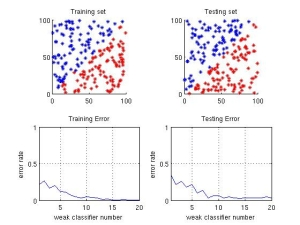
\includegraphics[width=0.8\textwidth]{chap2/adaboost}
    \bicaption[fig:adaboost]{Adaboost算法示例}{Adaboost算法示例}{Fig.}{Adaboost Example}
\end{figure}

\begin{figure}[!htp]
    \centering
    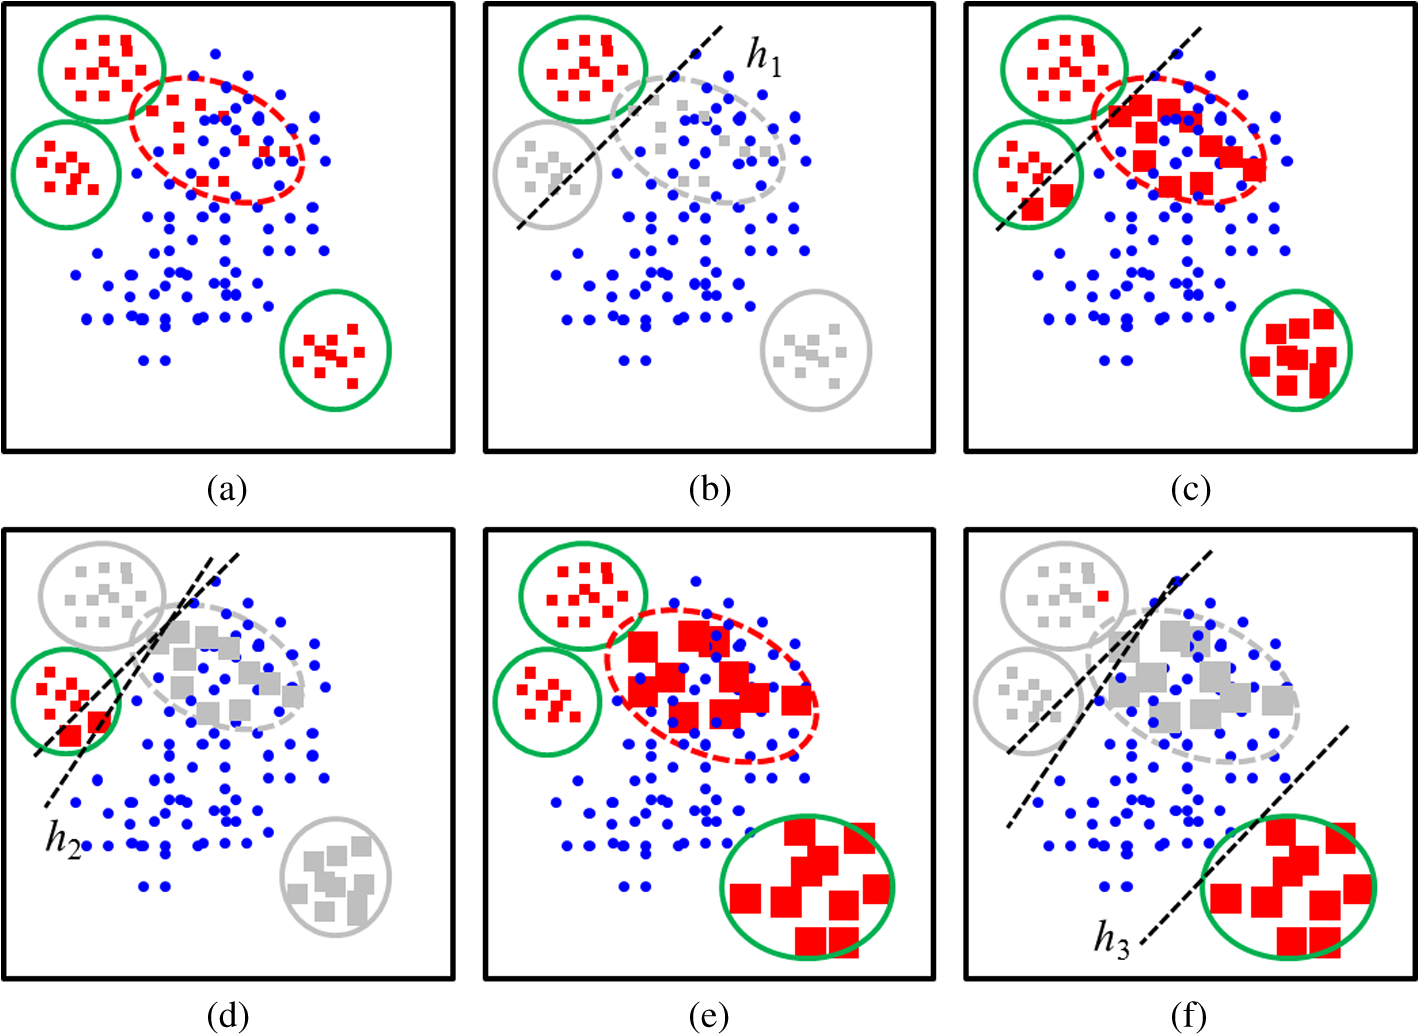
\includegraphics[width=0.8\textwidth]{chap2/adaboost2}
    \bicaption[fig:adaboost2]{Adaboost算法示例}{Adaboost算法示例}{Fig.}{Adaboost Example}
\end{figure}

\begin{algorithm}
    \caption{Adaboost}
    \label{algo:ada}
    \begin{algorithmic}[1]
    \State initial $D \gets \{ x^1, x^2, ..., x^n, y_{1}, y_{2}, ..., y_{n}\}, k_{max}$
    \State initial $W_{k}(i) \gets \frac{1}{n}, i=1,...,n$
    \For{$k = 1 \to k_{max}$}
        \State $k \gets k+1$
        \State 训练使用按照$W_{k}(i)$采样的$D$的弱学习器$C_{k}$
        \State $E_{k} \gets$对使用$W_{k}(i)$的$D$测量的$C_{k}$的训练误差 
        \State $\alpha_{k} \gets \frac{1}{2}ln\frac{1-E_{k}}{E_{k}}$
        \State $W_{k+1}(i) \gets \frac{W_{k}(i)}{Z_{k}} \times \begin{cases}
            e^{-\alpha_{k}}, & if h_{k}(x^i)=y_{i} \\
            e^{-\alpha_{k}}, & if h_{k}(x^i)\neq y_{i}
        \end{cases}$
    \EndFor
    \State 
    \Return $C_{k},\alpha_{k},k=1,...,k_{max}$
    \end{algorithmic}
\end{algorithm}

随机森林是适合于数据集的各种子样本上的多个决策树分类器,并且使用平均算法以提高预测精度和控制过拟合。我们假设用户知道单个分类树的构造,随机森林生长许多分类树。要从输入向量中分类新对象,请将输入向量放在森林中的每个树上。每棵树给出一个分类,我们说树的“投票”为该类。森林选择具有最多票数的分类(在森林中的所有树上)。

每棵树生长如下:
\begin{enumerate}
    \item 如果训练集中的数量为$N$,则从原始数据中随机抽样$N$个样本,但是要替换原始数据,该样本将是用于生长树的训练集。
    \item 如果存在$M$个输入变量,并且指定数目$m \ll M$,使得在每个节点处从$M$中随机选择$m$个变量,并且使用这些$m$上的最佳分割来分割节点,需要保持在森林生长期间$m$的值保持不变。
    \item 每棵树最大程度的生长,并且不经过修剪过程。
\end{enumerate}

在随机森林的原始论文中,表明森林错误率取决于两件事,即森林中任意两棵树之间的相关性,增加相关性增加森林错误率;森林中每棵树的强度,具有低错误率的树是强分类器,增加单个树的强度降低了森林错误率。减少$m$减小相关性和强度。增加它增加两者,中间的某处是$m$的“最佳”范围,通常来说$m$的最佳范围相当宽。使用out-of-bag错误率,可以快速找到范围内的$m$值,这是随机森林的唯一可调参数。

在随机森林中,不需要交叉验证或单独的测试集来获得测试集误差的无偏估计。在运行期间内部估计如下,每个树使用来自原始数据的不同引导样本来构造。大约三分之一的案例被排除在引导样本之外,而不用于第$k$棵树的构建。将所有使用第$k$个树构造的样本,放在第$k$个树上进行分类。以这种方式,对于每种情况在大约三分之一的树中获得测试集分类。在运行结束时令$j$记为获得大部分投票的类。$j$非真的比例的平均值即为out-of-bag误差。这在许多测试中被证明是公正的。

绝大多数的决策树算法都要进行重要的剪枝步骤,但是随机森林模型并不需要进行剪枝操作,由于之前的行采样和列采样过程保证了样本的随机性,也不太容易出现过拟合的现象。

另外随机森林算法是可以通过行化来提升性能,但是Adaboost模型无法并行。图\ref{fig:rf}即为随机森林示例:

\begin{figure}[!htp]
    \centering
    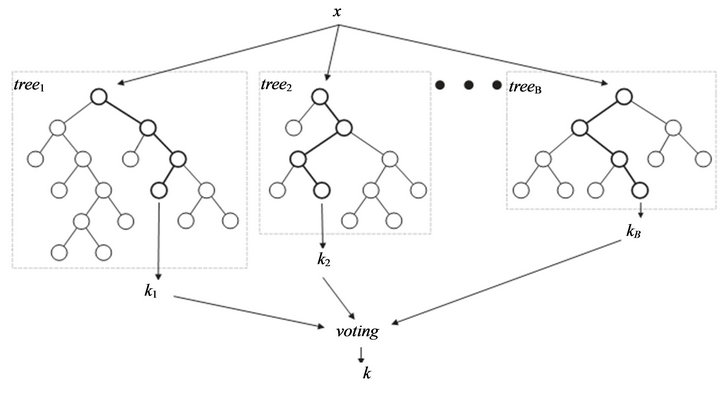
\includegraphics[width=0.8\textwidth]{chap2/rf}
    \bicaption[fig:rf]{Random Forest算法示例}{Random Forest算法示例}{Fig.}{Random Forest Example}
\end{figure}

最后,对于Gradient Boosting Decision Tree算法,该模型的每一次计算都减少了上一次训练模型的残差,而为了减少这些残差对模型的影响,可以在残差减少的梯度方向上建立一个新模型。这与Adaboost和随机森林算法之间有显著差异。

\section{自动编码器}

神经网络(Neural network)是一种基于大量神经单元集合的计算方法,松散地建模生物大脑,用于解决由轴突连接的生物神经元的大群集的问题。每个神经单元与许多其他神经单元连接在一起,并且如果神经单元处于激活状态,那么链接可以在它们对所连接的神经元的中实施影响或抑制神经元。每个单独的神经单元可以具有将所有其输入的值组合在一起求和的功能。在每个链接或者单元本身上可以存在阈值函数,使得它必须在传播到其他神经元之前超过阈值。这些系统是自学习和训练的而不是明确编程的,神经网络在传统计算机程序中难以解决的问题或者特征检测的领域中有着优异的表现。如图\ref{fig:neurons}是一个小神经网络。

\begin{figure}[!htp]
    \centering
    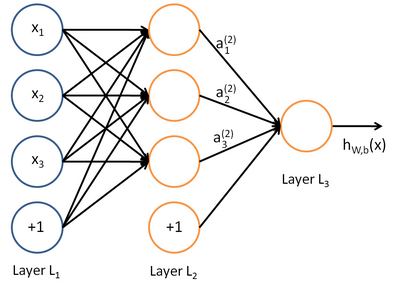
\includegraphics[width=0.8\textwidth]{chap2/neurons}
    \bicaption[fig:neurons]{神经网络模型}{神经网络模型}{Fig.}{Neural Network}
\end{figure}
在图\ref{fig:neurons}中,我们使用圆圈也表示网络的输入。标记为“+1”的圆圈被称为偏移单元,并且对应于截距项。网络的最左层称为输入层,最右层是输出层,在这个例子中其仅具有一个输出节点。中间层的节点被称为隐藏层,因为这些节点的值在训练集中没有被观察到。我们可以得到如下结论,示例神经网络有3个输入单位,3个隐藏单位和1个输出单位。

我们将让$n_l$表示网络中的层数。我们将层$l$标记为$L_1$,因此层$L_1$是输入层,层$L_{n_{l}}$是输出层。我们的神经网络具有参数$(W,b)=(W^{(1)},b^{(1)},W^{(2)},b^{(2)})$,其中我们认为$W ^ {(l)} _ {ij}$与层1中的单元$j$和层$l + 1$中的单元$i$之间的连接相关联的参数(或权重)。此外,$b ^ {(1)}$是$i$单元在第$j+1$层的偏移单元。因此,在我们的示例中$W^{(1)} \in \Re^{3\times 3}$并且$ W^{(2)} \in \Re^{1\times 3}$。注意偏置单元没有输入或连接到它们,因为它们总是输出值+1。我们还让$s_l$表示层$l$中的节点数量。
我们将层$l$中单元$i$激活得到$ W^{(1)} \in \Re^{3\times 3} $。对于$l = 1$,我们还使用$a^{(1)}_i = x_i$表示第$i$个输入。在给定参数$W$,$b$时,我们的神经网络定义输出实数为$h_{W,b}(x)$。具体地,该神经网络表示的计算由式\ref{eq:neursons}给出:

{\setlength\abovedisplayskip{15pt}
\setlength\belowdisplayskip{15pt}
\begin{eqnarray}
    \label{eq:neursons}
    a_1^{(2)} = f(W_{11}^{(1)}x_1 + W_{12}^{(1)} x_2 + W_{13}^{(1)} x_3 + b_1^{(1)})  \nonumber \\
    a_2^{(2)} = f(W_{21}^{(1)}x_1 + W_{22}^{(1)} x_2 + W_{23}^{(1)} x_3 + b_2^{(1)})  \nonumber \\
    a_3^{(2)} = f(W_{31}^{(1)}x_1 + W_{32}^{(1)} x_2 + W_{33}^{(1)} x_3 + b_3^{(1)})  \\
    h_{W,b}(x) = a_1^{(3)} =  f(W_{11}^{(2)}a_1^{(2)} + W_{12}^{(2)} a_2^{(2)} + W_{13}^{(2)} a_3^{(2)} + b_1^{(2)}) \nonumber
\end{eqnarray}}

我们使用$z^{(l)}_i $表示单元$i$在$l$层的总权重,所以我们有$a^{(l)}_i = f(z^{(l)}_i)$。带入到\ref{eq:neursons}中化简得\ref{eq:neursons2}:

{\setlength\abovedisplayskip{15pt}
\setlength\belowdisplayskip{15pt}
\begin{eqnarray}
    \label{eq:neursons2}
    z^{(2)} = W^{(1)} x + b^{(1)}  \nonumber \\
    a^{(2)} = f(z^{(2)})  \nonumber \\
    z^{(3)} = W^{(2)} a^{(2)} + b^{(2)}  \\
    h_{W,b}(x) = a^{(3)} = f(z^{(3)})  \nonumber
\end{eqnarray}}

通过在矩阵中组织我们的参数和使用矩阵向量操作,我们可以利用快速线性代数例程在我们的网络中快速执行计算。图\ref{fig:multi-neurons}是一个多层的神经网络。

\begin{figure}[!htp]
    \centering
    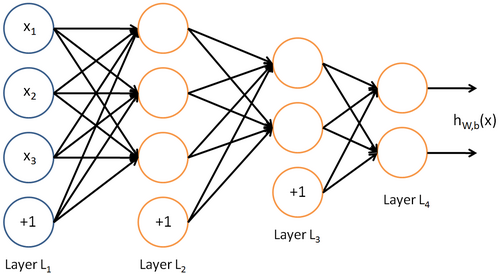
\includegraphics[width=0.8\textwidth]{chap2/multi-neurons}
    \bicaption[fig:multi-neurons]{多层神经网络}{多层神经网络}{Fig.}{Multi Layer Neural Network}
\end{figure}

我们已经描述了神经网络的监督学习的应用,其中我们标记了训练示例。 现在假设我们只有一组未标记的训练样本$\{x^{(1)}, x^{(2)}, x^{(3)}, \ldots\}$,其中$ x^{(i)} \in \Re^{n}$。 自动编码器神经网络是应用反向传播的无监督学习算法,将目标值设置为等于输入。 即它使用$y^{(i)} = x^{(i)}$。图\ref{fig:autoencoder}即为自动编码算法示例。

\begin{figure}[!htp]
    \centering
    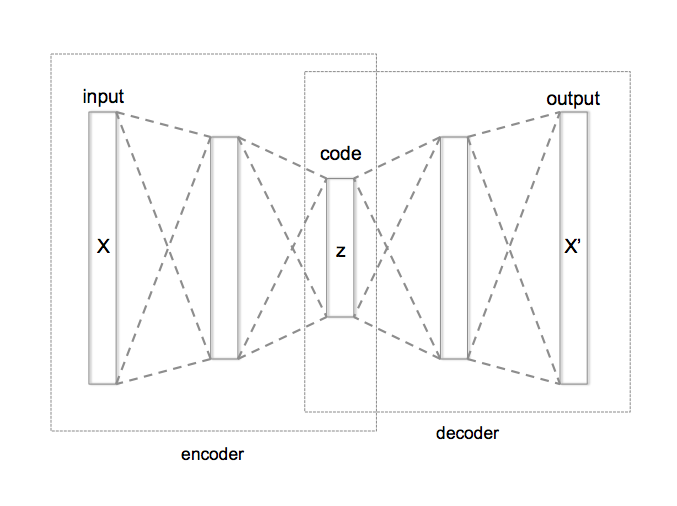
\includegraphics[width=0.8\textwidth]{chap2/autoencoder}
    \bicaption[fig:autoencoder]{自动编码器}{自动编码器}{Fig.}{Autoencoder}
\end{figure}

自动编码器尝试学习函数$e h_{W,b}(x) \approx x$。即试图学习身份函数的近似,以便输出类似于$x$的$\hat{x}$。身份函数是通过在网络上设置约束,例如通过限制隐藏单元的数量,我们可以发现隐藏的数据结构。在结构上,自动编码器的最简单形式是非常类似于多层感知器(英文:multilayer perceptron,缩写:MLP)的前馈非反复神经网络,具有输入层,输出层和连接它们的一个或多个隐藏层,但是具有输出层具有与输入层相同数量的节点,并且具有重建其自己的输入的目的。因此,自动编码器是无监督的学习模型。自动编码器总是由两部分组成,即编码器和解码器,可以定义为$\phi$和$\psi$。所以有\ref{eq:phi}

{\setlength\abovedisplayskip{15pt}
\setlength\belowdisplayskip{15pt}
\begin{eqnarray}
    \label{eq:phi}
    \phi :{\mathcal {X}}\rightarrow {\mathcal {F}} \nonumber \\
    \psi :{\mathcal {F}}\rightarrow {\mathcal {X}} \\
    \arg \min _{\phi ,\psi }\|X-(\psi \circ \phi )X\|^{2} \nonumber
\end{eqnarray}}

在简单的情况中只有一层隐藏层,自动编码器的输入$\mathbf {x} \in \mathbb {R} ^{d}={\mathcal {X}}}$映射成$\mathbf {z} \in \mathbb {R} ^{p}={\mathcal {F}}$。\ref{eq:phi2}

{\setlength\abovedisplayskip{15pt}
\setlength\belowdisplayskip{15pt}
\begin{equation}
    \label{eq:phi2}
    \mathbf {z} =\sigma _{1}(\mathbf {Wx} +\mathbf {b} )
\end{equation}}

这通常被称为代码或潜在变量,这里$\sigma _ {1}$是元素方式的激活函数,例如$S$形函数或整流线性单元。之后,$\mathbf {z}$映射到重构$\mathbf {x'}$的形状相同$\mathbf {x}$,如式\ref{eq:phi3}所示:

{\setlength\abovedisplayskip{15pt}
\setlength\belowdisplayskip{15pt}
\begin{equation}
    \label{eq:phi3}
   \mathbf {x'} =\sigma _{2}(\mathbf {W'z} +\mathbf {b'} )
\end{equation}}

自动编码器也被训练以最小化重建误差\ref{eq:phi4}:

{\setlength\abovedisplayskip{15pt}
\setlength\belowdisplayskip{15pt}
\begin{equation}
    \label{eq:phi4}
    {\mathcal {L}}(\mathbf {x} ,\mathbf {x'} )=\|\mathbf {x} -\mathbf {x'} \|^{2}=\|\mathbf {x} -\sigma _{2}(\mathbf {W'} (\sigma _{1}(\mathbf {Wx} +\mathbf {b} ))+\mathbf {b'} )\|^{2}
\end{equation}}

如果特征空间${\mathcal {F}}$具有比输入空间更小的维度{\mathcal {X}},然后是特征向量$\phi(x)$可以被看作是输入的压缩表示$X$。 如果隐藏层大于输入层,则自动编码器可能潜在地学习身份功能并变得无用。然而实验结果表明,自动编码器在这些情况下仍然可以学习有用的功能\cite{bengio2009learning}。

自动编码器的训练算法可以概括为:对于每个输入$x$,执行前馈传递以计算所有隐藏层的激活,然后在输出层获取输出\mathbf{x'}测量的偏差\mathbf {x'},通过网络反向传播错误并执行重量更新。

自动编码器经常使用反向传播的许多变体之一(诸如共轭梯度法,最速下降法等)来训练。虽然这些通常是相当有效的,但是使用反向传播来训练具有许多隐藏层的网络存在根本问题。一旦错误反向传播到前几层,它们会变得不重要。这意味着网络几乎总是学会重建所有训练数据的平均值。虽然更高级的反向传播方法(如共轭梯度法)可以在一定程度上解决这个问题,但是它们仍然导致非常缓慢的学习过程和解决方案。这个问题可以通过使用近似最终解的初始权重来补救。找到这些初始权重的过程通常被称为预训练。

Geoffrey Hinton开发了一种用于训练多层深自动编码器的预训练技术。这种方法包括将每一组相邻的两层作为受限的波尔兹曼机器\cite{smolensky1986information},使得预训练接近良好的解,然后使用反向传播技术来微调结果。这个模型取名为深信仰网络(deep belief network)\cite{hinton2009deep}。

\section{本章小结}

在本章节中我们分别对本文中涉及到的算法、模型以及相应的技术进行了全方位的介绍。

首先是对3GPP Release9标准当中定义的三种定位算法(E-CellID, OTDOA, A-GNSS)进行了详细的比较。特性分别是:

\begin{enumerate}
    \item \textbf{E-CellID} 通过实验可以得到基于E-CellID的定位精度是,67\%的设备定位精度在80m和95\%的设备定位精度在170m左右,而根据3GPP规范,该方法的标称(90\%)测量精度为78m。E-CellID的优势在于不受环境的限制即可完成定位,并且无需用户侧安装第三方的应用,只要是使用LTE协议的手持设备即可达到定位的目的。
    \item \textbf{OTDOA} OTDOA位置精度主要取决于RSTD质量和几何形状。实验表明50\%的测量结果误差在20m左右和95\%的测量误差在63m以内。但是这组实验结果是在信道、物理环境均在较为理想的环境下实验所得,在更复杂、信号更不稳定的无线环境中,精度可能会大幅降低。OTDOA技术相较于E-CellID技术定位精度更高,但是受环境制约较多,由于其原理是根据信号达到时间差来计算用户设备的位置,所以至少需要三个基站同时定位才能达到定位的目的。
    \item \textbf{A-GNSS} A-GPS和A-GNSS的性能主要取决于卫星定位的性能,并且已知这些方法在空旷野外的条件下非常准确,然而在密集的城市中,由于存在非常高的建筑物导致定位精度显著下降。并且由于是使用卫星定位的技术,并不是本课题研究的重点内容。
\end{enumerate}

本章节的第二部分对人群移动模型研究的意义和在本文中的作用进行了分析。在突发紧急事件人群需要撤离的情况下,针对人群移动模型的研究工作显得非常重要。在本章节中对基于社会关系的人群移动模型和元胞自动机模型进行了分析回归,从数学角度对这两种模型进行了阐述。

本章节的第三部分对决策树模型从原理上进行了分析与归纳。在决策树模型中最重要的三个步骤分别是

\begin{enumerate}
    \item 特征选择
    \item 决策树生成算法
    \item 剪枝算法
\end{enumerate}
而评价一颗决策树的方法就是通过数据纯度函数进行评价,其中常用的三种方法分别是信息增益、基尼指数和方差减小三种模型。决策树的优势在于易于理解和实现,能够快速的得到结果。但是决策树模型很容易出现过拟合现象,要避免这个问题剪枝机制是必要的。在这种情况下,决策树变得非常大。解决问题的方法包括改变问题域的表达方式或使用更具表现力的模型的学习算法。

本文的研究内容最终会使用到机器学习的算法对未来人群分布进行预测,所以在本章节的第三部分对基于决策树的梯度迭代决策树(英文:Gradient Boosting Decision Tree,缩写:GBDT)进行了从原理到算法层面的全方位的分析,并且与其他的基于决策树的回归算法进行了对比。

在讨论了有监督学习的算法之后,我们将使用无监督学习对人群分步进行预测,所以在第四部分对自动编码器进行了较为全面的介绍。自动编码器是基于机器学习算法,在神经网络中将输入和输出均置为已经提取到的特征,经过神经网络的学习之后我们可以找到这些特征之间隐藏的关联,从而就得到了模型中新的特征。